\documentclass[a4paper,11pt,final]{book}

\usepackage[utf8]{inputenc} 
\usepackage[T1]{fontenc}

\usepackage{lmodern}

\usepackage{graphicx}
\graphicspath{{.}{../book-result/Slides/Handout/}}

\usepackage{tikz}

\usepackage{calc}

\usepackage{xspace}

\usepackage[absolute,overlay]{textpos} 

\usepackage{url}

\usepackage[unicode]{hyperref}

\hypersetup{
	colorlinks,
	menucolor=black,
	urlcolor=black,
	linkcolor=black,
	pdftitle={Pharo MOOC}, 
    pdfauthor={Damien Cassou, Stéphane Ducasse and Luc Fabresse}
}

\setlength{\pdfpagewidth}{210mm} 
\setlength{\pdfpageheight}{297mm}
\usepackage[a4paper,pdftex,twoside,nomarginpar,inner=20mm,outer=20mm,top=20mm,bottom=20mm]{geometry}



\usepackage{minitoc}

\usepackage{tocloft}

\renewcommand{\cftchapfont}{\bfseries}
\renewcommand{\cftchappagefont}{\bfseries}
\renewcommand{\cftchappresnum}{Week }
\renewcommand{\cftchapaftersnum}{:}
\renewcommand{\cftchapnumwidth}{5em}



\usepackage[final]{pdfpages}

%
% Boxed environment with semi-transparent shadow.
% http://www.texample.net/tikz/examples/transparent-shadows/
\newlength{\boxw}
\newlength{\boxh}
\newlength{\shadowsize}
\newlength{\boxroundness}
\newlength{\tmpa}
\newsavebox{\shadowblockbox}

\setlength{\shadowsize}{6pt}
\setlength{\boxroundness}{3pt}

\newenvironment{shadowblock}[1]%
{\begin{lrbox}{\shadowblockbox}\begin{minipage}{#1}}%
{\end{minipage}\end{lrbox}%
\settowidth{\boxw}{\usebox{\shadowblockbox}}%
\settodepth{\tmpa}{\usebox{\shadowblockbox}}%
\settoheight{\boxh}{\usebox{\shadowblockbox}}%
\addtolength{\boxh}{\tmpa}%
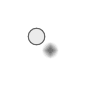
\begin{tikzpicture}
    \addtolength{\boxw}{\boxroundness * 2}
    \addtolength{\boxh}{\boxroundness * 2}

    \foreach \x in {0,.05,...,1}
    {
        \setlength{\tmpa}{\shadowsize * \real{\x}}
        \fill[xshift=\shadowsize - 1pt,yshift=-\shadowsize + 1pt,
                black,opacity=.04,rounded corners=\boxroundness]
            (\tmpa, \tmpa) rectangle +(\boxw - \tmpa - \tmpa,
                \boxh - \tmpa - \tmpa);
    }

    \filldraw[fill=black!08, draw=black!60, rounded corners=\boxroundness]
        (0, 0) rectangle (\boxw, \boxh);
    \draw node[xshift=\boxroundness,yshift=\boxroundness,
        inner sep=0pt,outer sep=0pt,anchor=south west]
             (0,0) {\usebox{\shadowblockbox}};
\end{tikzpicture}}



% C019SD-W1S01-blabla
% e.g. \includehandoutfile{W1S01}{Basic-ArraySetOrderedCollection}{Video 5min}
\newcommand{\includehandoutfile}[3]{%
% \section*{[#3] #2}
\addcontentsline{toc}{section}{[#3] #2}
\phantomsection%
\includepdf[pages={-},pagecommand={\markboth{#1-#2}{#1-#2}},link,templatesize={19cm}{24.5cm}]{#2-Handout}
% 
}


% e.g. \externalresource{W1S01}{Implementing a Counter}{Live 5min}
\newcommand{\externalresource}[3]{%
\markboth{#2}{#3}
% \phantomsection%
\addcontentsline{toc}{section}{[#3] #2}
% \section*{[#3] #2}
}

\renewcommand{\chaptername}{Week}

\newcommand{\week}[1]{%
\chapter{#1}
% \addcontentsline{toc}{chapter}{Week #1}
\minitoc
}

\begin{document}

\thispagestyle{empty}
\begin{center}
	\vspace*{1em}

	~\vfill %%%
	
	\begin{shadowblock}{\linewidth}
		\centering
		\begin{minipage}{\linewidth}
		\noindent\vspace*{1em}
		\begin{center}
		\textbf{\Huge Pharo MOOC}
		
		\vspace*{3.5em}
	
		{\LARGE Damien Cassou, Stéphane Ducasse and Luc Fabresse}
      
      \vspace*{2em}
      
      2015\\  
      \vspace*{0.5em}
	\end{center}    
	 
      \vspace*{1em}
	\end{minipage}
	\end{shadowblock}
\end{center}

~\vfill %%%

\newpage

\chapter*{About this MOOC}

This document summarizes the whole MOOC planning week by week.
In the outline, you will see that 4 kind of activities are distinguished:

\begin{description}
\item[Video] means that you should watch a video explaining some notions described in slides.
You will find a handout version of all slides in this document. 
We invite you to always watch videos while taking notes on the slides.

\item[Live] means that should watch a video demonstrating a coding session in Pharo. 

\item[Redo] means that you should watch a Live and redo by yourself in Pharo what has been demonstrated.

\item[Todo] means that you shall do an exercice by yourself in Pharo.

\end{description}

\newpage

\dominitoc
\tableofcontents

\newpage

% =======================
\week{Welcome on Board and Syntax Discovery}
% =======================

% \includehandoutfile{W1S01}{ObjectivesCourse}{Video 6min}  %OLD
% \includehandoutfile{W1S01}{ObjectivesMooc}{Video 6min}    %OLD

\includehandoutfile{W1S01}{Intro-ObjectivesMooc}{Video 2min}
\includehandoutfile{W1S02}{Intro-WhatIs}{Video 6min}
\includehandoutfile{W1S03}{Intro-Vision}{Video 6min}
\externalresource  {W1S04}{Pharo install and Hello World example}{Live 6min}
\includehandoutfile{W1S05}{Intro-ModelInaNushell}{Video 6min}
\includehandoutfile{W1S06}{Intro-SyntaxInANutshell}{Video 6min}
\externalresource  {W1S07}{Runtime: The notion of image, saving code}{Live 6min}

\externalresource  {W1S08}{Coding a Counter}{Redo 6min}
\externalresource  {W1S09}{Coding a Counter: the Pharo way}{Redo 6min}
\externalresource  {W1S10}{Coding a REST interface to a counter}{Redo 6min}
\externalresource  {W1S11}{Lamp et FeuTricolor}{Todo}

% =======================
\week{The Complete Pharo Syntax}
% =======================

\includehandoutfile{W2S01}{Messages}{Video 6min}
\includehandoutfile{W2S02}{Messages-ForTheJavaProgrammers}{Video 6min}
\includehandoutfile{W2S03}{Messages-Precedence}{Video 6min}
\includehandoutfile{W2S04}{Messages-Sequence}{Video 6min}

\externalresource  {W2S05}{Inspecting a Counter}{Live 6min}
\externalresource  {W2S06}{Publishing Code on smalltalkhub.com}{Live 6min}

\includehandoutfile{W2S07}{Blocks}{Video 6min}
\includehandoutfile{W2S08}{Blocks-Loops}{Video 6min}
\includehandoutfile{W2S09}{Basic-Loops}{Video 6min}

\includehandoutfile{W2S10}{Basic-BooleansAndCondition}{Video 6min}
\includehandoutfile{W2S11}{Message-ParenthesisVsSquareBrackets}{Video 6min}


% Exo 
\externalresource  {W2S12}{Simple Exos Syntax}{Todo}
\externalresource  {W2S13}{Exos on Loops}{Todo}
\externalresource  {W2S14}{Coding a moving Turtle}{Redo}

\externalresource  {W2S15}{Coding a Ticket Model}{Todo}
\includehandoutfile{W2S16}{Design-EssenceOfDispatchExo}{Video / Exo}

\end{document}

% =======================
\week{3}
% =======================

\includehandoutfile{W1S02}{Basic-ArraySetOrderedCollection}{Video 6min}
\includehandoutfile{W1S01}{AdvancedDidYouReallyUnderstandSuper}{Video 6min}
\includehandoutfile{W1S01}{Basic-ArraySetOrderedCollection}{Video 6min}

\includehandoutfile{W1S01}{Basic-ClassAndMethodDefinition}{Video 6min}
\includehandoutfile{W1S01}{Basic-ClassMethods}{Video 6min}
\includehandoutfile{W1S01}{Basic-ClassMethodsAtWork}{Video 6min}
\includehandoutfile{W1S01}{Basic-Exceptions}{Video 6min}

\includehandoutfile{W1S01}{Basic-Numbers}{Video 6min}
\includehandoutfile{W1S01}{Basic-RuntimeArchitecture}{Video 6min}
\includehandoutfile{W1S01}{Basic-Streams}{Video 6min}
\includehandoutfile{W1S01}{Basic-Variables}{Video 6min}

\includehandoutfile{W1S01}{Design-AboutFinalAndOthers}{Video 6min}
\includehandoutfile{W1S01}{Design-AvoidIsNil}{Video 6min}
\includehandoutfile{W1S01}{Design-ClassAsObjects}{Video 6min}
\includehandoutfile{W1S01}{Design-EssenceOfDispatch}{Video 6min}

\includehandoutfile{W1S01}{Design-HookAndTemplate}{Video 6min}

% =======================
\week{4}
% =======================

\includehandoutfile{W1S01}{Design-HooksAndTemplate}{Video 6min}
\includehandoutfile{W1S01}{Design-LibrariesVsFrameworks}{Video 6min}
\includehandoutfile{W1S01}{Design-SelfSendsArePlanForReuse}{Video 6min}
\includehandoutfile{W1S01}{Design-WhyTesting}{Video 6min}
\includehandoutfile{W1S01}{InheritanceAndLookup-1-Inheritance}{Video 6min}

% =======================
\week{5}
% =======================

\includehandoutfile{W1S01}{InheritanceAndLookup-2-Lookup}{Video 6min}
\includehandoutfile{W1S01}{InheritanceAndLookup-3-Super}{Video 6min}
\includehandoutfile{W1S01}{InheritanceAndLookup-4-DoesNotUnderstand}{Video 6min}
\includehandoutfile{W1S01}{InheritanceAndLookup-5-LookupMetaclasses}{Video 6min}


% =======================
\week{6}
% =======================

\includehandoutfile{W1S01}{Intro-SyntaxInANutshell-newVersion}{Video 6min}
\includehandoutfile{W1S01}{Iterators}{Video 6min}


% =======================
\week{7}
% =======================

\includehandoutfile{W1S01}{TeapotServer}{Video 6min}
\includehandoutfile{W1S01}{TestAdvocado}{Video 6min}


\end{document}

  
